\documentclass{article}
\usepackage{color}
\usepackage{alltt}
\usepackage[T1]{fontenc}
%\usepackage[latin1]{inputenc}
\usepackage[ngerman]{babel}
\usepackage{graphicx}
\usepackage{hyperref}
\graphicspath{ {./images/} }

% Style definition file generated by highlight 4.2, http://www.andre-simon.de/ 
% highlight theme: Kwrite Editor
\newcommand{\hldef}[1]{\textcolor[rgb]{0,0,0}{#1}}
\newcommand{\hlnum}[1]{\textcolor[rgb]{0.69,0.49,0}{#1}}
\newcommand{\hlesc}[1]{\textcolor[rgb]{1,0,1}{#1}}
\newcommand{\hlsng}[1]{\textcolor[rgb]{0.75,0.01,0.01}{#1}}
\newcommand{\hlpps}[1]{\textcolor[rgb]{0.51,0.51,0}{#1}}
\newcommand{\hlslc}[1]{\textcolor[rgb]{0.51,0.51,0.51}{\it{#1}}}
\newcommand{\hlcom}[1]{\textcolor[rgb]{0.51,0.51,0.51}{\it{#1}}}
\newcommand{\hlppc}[1]{\textcolor[rgb]{0,0.51,0}{#1}}
\newcommand{\hlopt}[1]{\textcolor[rgb]{0,0,0}{#1}}
\newcommand{\hlipl}[1]{\textcolor[rgb]{0,0.34,0.68}{#1}}
\newcommand{\hllin}[1]{\textcolor[rgb]{0.33,0.33,0.33}{#1}}
\newcommand{\hlerr}[1]{\textcolor[rgb]{1,0,0}{\bf{#1}}}
\newcommand{\hlerm}[1]{\marginpar{\small\itshape\color{red}#1}}
\newcommand{\hlkwa}[1]{\textcolor[rgb]{0,0,0}{\bf{#1}}}
\newcommand{\hlkwb}[1]{\textcolor[rgb]{0,0.34,0.68}{#1}}
\newcommand{\hlkwc}[1]{\textcolor[rgb]{0,0,0}{#1}}
\newcommand{\hlkwd}[1]{\textcolor[rgb]{0,0,0.51}{#1}}
\newcommand{\hlkwe}[1]{\textcolor[rgb]{0.05,0.36,0.76}{#1}}
\newcommand{\hlkwf}[1]{\textcolor[rgb]{0.46,0.05,0.76}{#1}}
\definecolor{bgcolor}{rgb}{0.88,0.92,0.93}



\title{api_dokumentation}
\begin{document}
% \pagecolor{bgcolor}
\section{Wie tauschen wir Daten zwischen unserem Client und unserem Server aus?}
Wir benutzen eine RestAPI um über das HTTP-Protokol Daten 
zwischen unserem Server und unserem Client auszutauschen.

In einer RestAPI werden die CRUD-Operationen durch 
HTTP-Request Methoden dargestellt.

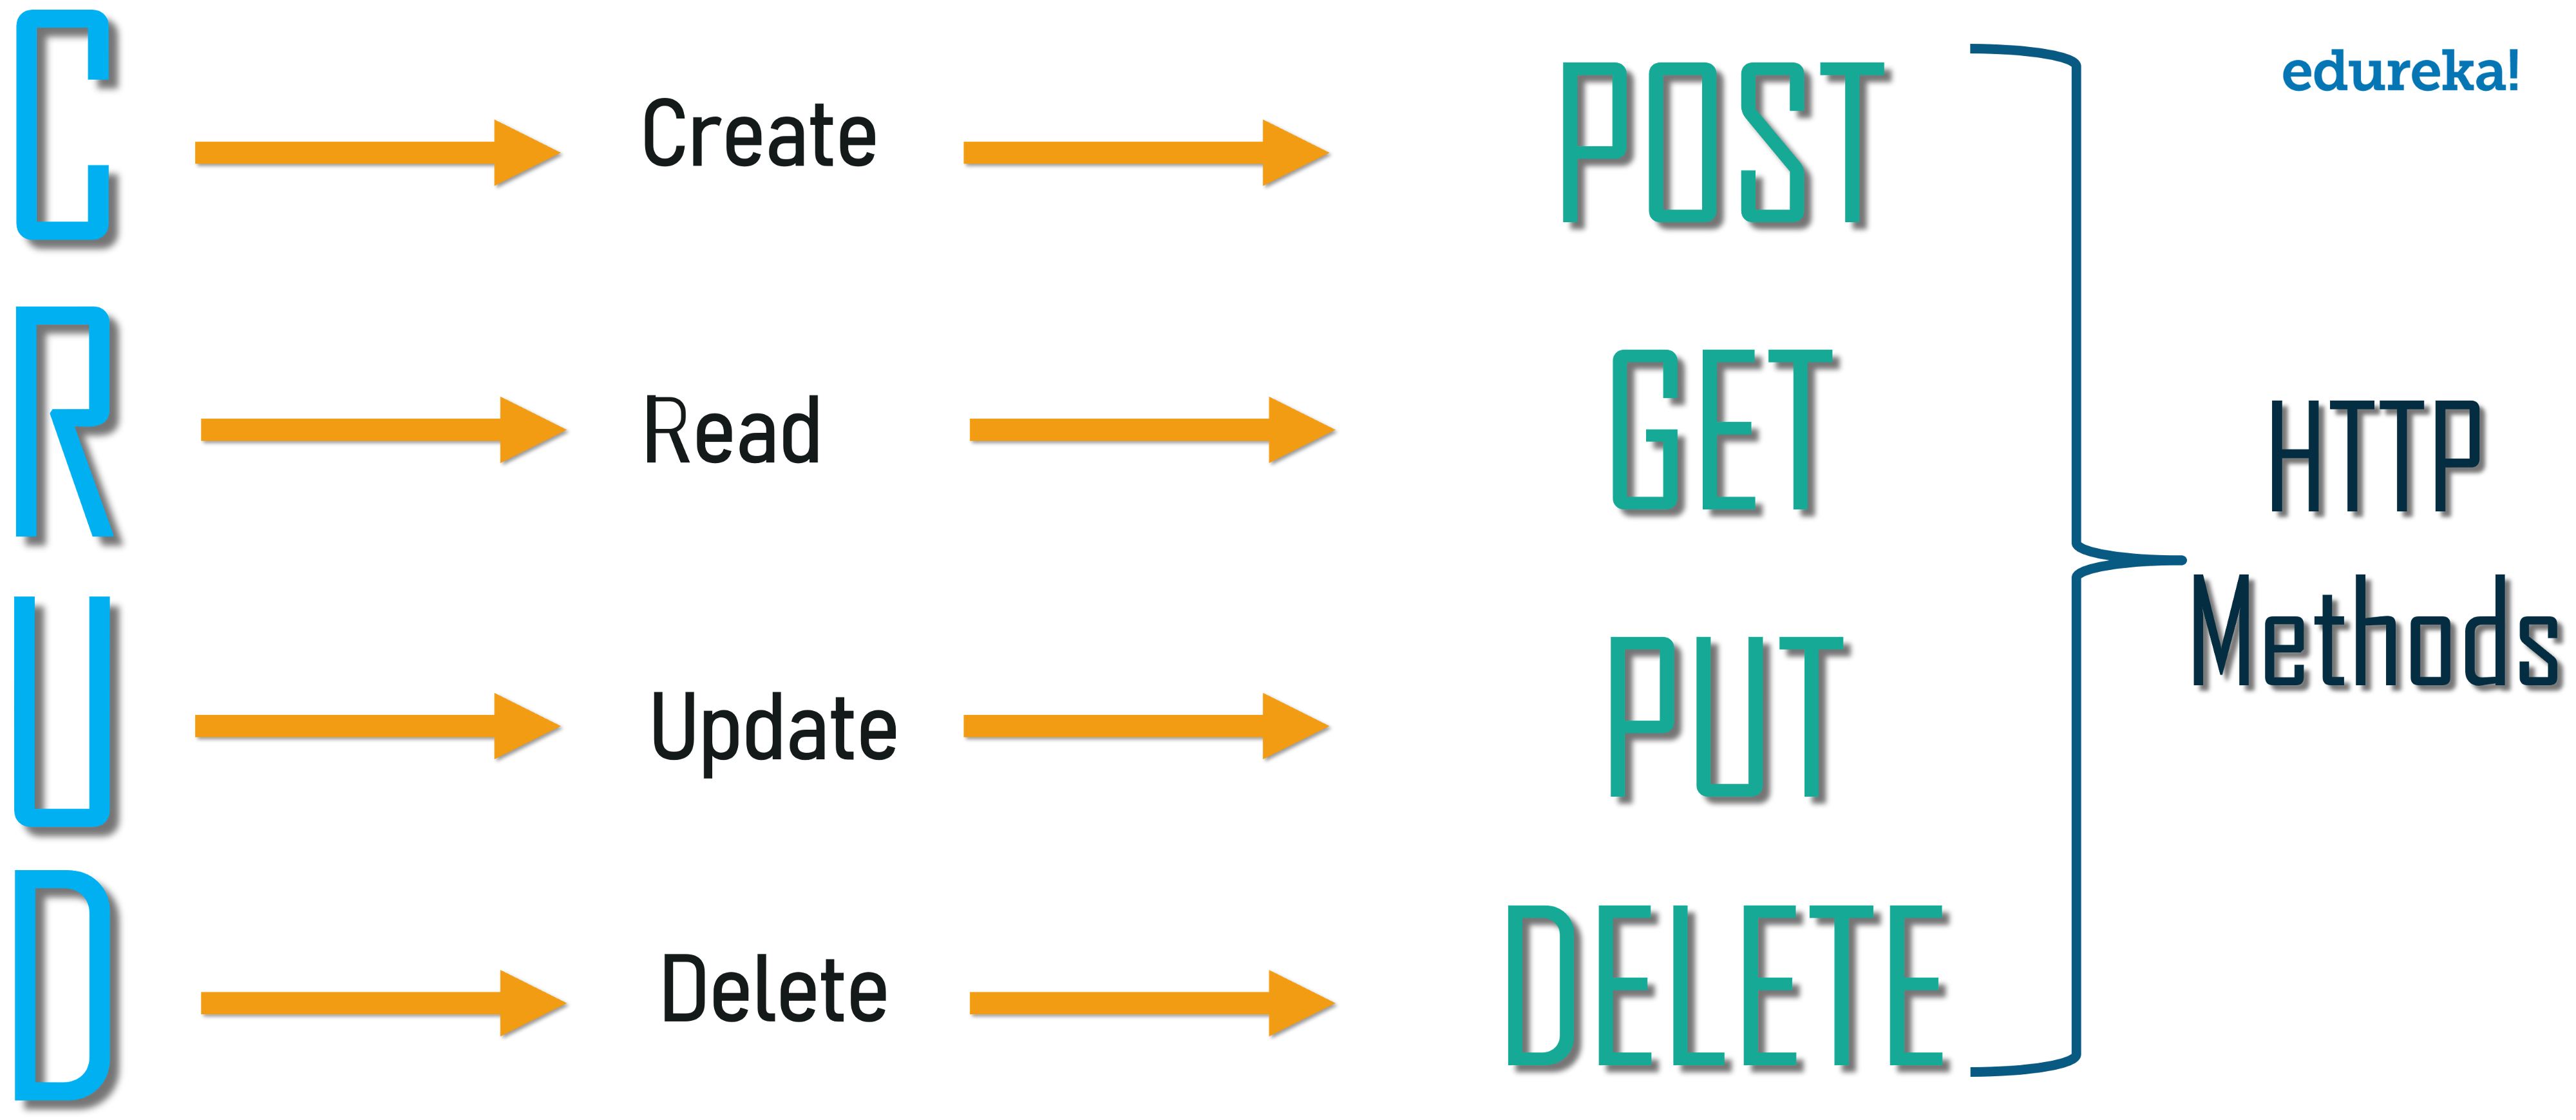
\includegraphics[width=\textwidth]{crud_to_http.png}

\subsection{Beispiel Benutzer erstellen}

Es werden an verschiedene API-Endpunkte Anfragen gestellt um Daten auf dem Server zu verwalten.
Um beispielsweise einen Benutzer zu erstellen, wird ein POST-Request an den API-Endpunkt /users gesendet.

\begin{verbatim}
    POST: [api-url]/users
\end{verbatim}

Damit ein neuer Nutzer erstellt werden kann, werden weitere informationen benötigt.
Diese können entweder als Parameter in der URL eingefügt werden oder im JSON-Format als Payload
mitgeschickt werden.

\subsubsection{Erstellen mit URL-Parametern}
Zum erstellen eines Nutzers sind beispielsweise ein Benutzername und ein Passwort nötig. Diese können als
Parameter in der URL mitgeschickt werden. Parameter werden an das Ende der URL eingefügt und beginnen hinter 
einem ?. Jeder weitere Parameter kann mit einem \&-Zeichen angehängt werden. In Beispiel des erstellen eines
Benutzers könnte eine Anfrage dann so aussehen:

\begin{verbatim}
    POST: [api-url]/users?username=max_musterman&password=bad_password
\end{verbatim}

\subsubsection{Erstellen mit JSON-Payload}
Alternativ kann auch ein JSON-Objekt mit an den Server gesendet werden. Die URL bleibt dann
bei [api-url]/users aber es wird der HTTP-Anfrage eine JSON-Objekt mitgegeben, welches in unserem Fall
so aussehen könnte:

\shorthandoff{"}
\noindent
\ttfamily
\hldef{}\hlkwa{\{}\hspace*{\fill}\\
\hldef{}\hldef{\ \ \ \ }\hldef{}\hlkwc{"username"}\hldef{}\hlopt{:\ }\hldef{}\hlsng{"max\textunderscore musterman"}\hldef{}\hlopt{,}\hspace*{\fill}\\
\hldef{}\hldef{\ \ \ \ }\hldef{}\hlkwc{"password"}\hldef{}\hlopt{:\ }\hldef{}\hlsng{"password"}\hldef{}\hspace*{\fill}\\
\hldef{}\hlkwa{\}}\hldef{}\hspace*{\fill}\\
\mbox{}
\normalfont
\normalsize
\shorthandon{"}

\subsubsection{Server Antwort}

Der Server muss auf diese Anfragen beantworten. Als erstes gibt es einen Antwortcode
welcher grundsätzlich Auskunft darüber gibt ob  die Anfrage erfolgreich beantwortet werden
konnte. In unsere Beispiel würde der Code 201 über das erfolgreiche erstellen eines neuen Benutzers
informieren. Alle möglichen Codes sind \href{https://developer.mozilla.org/en-US/docs/Web/HTTP/Status}{hier} von Mozilla
aufgelistet. Zusätzlich kann, wie bei der Anfrage auch, über JSON Informationen zurückgegeben
werden.

\subsection{Authentication}
Damit ein Benutzer nur seine Daten verändern kann, muss sichergestellt werden, dass der Nutzer auch das Recht hat
die HTTP-Anfrage zu stellen die er stellt. Damit ein Benutzer beweisen kann, dass er das Recht hat seine Daten zu verändern,
wird bei der Anfrage an den Server neben der URL und der Payload sogenannte HTTP-Header gesetzt.
Wir benutzen diese Header um einen String mitzuschicken, mit welchem wir beweisen, dass wir der Nutzer sind, 
welcher wir behaupten zu sein.

Diesen String bekommt man, indem man sich mit Benutzername und Passwort anmeldet. Dieser String
muss vom Client gespeichert werden, und wird jedes mal mitgeschickt, wenn eine Anfrage an den Server 
gestellt wird.

\section{Code Beispiel}

//TODO

\section{API Dokumentation}

Standart HTTP-Codes:
\begin{verbatim}
    200: OK
    201: Created
    400: Bad Request
    401: Unauthorized
    403: Forbidden
    500: Internal Server Error
    501: Not implemented
\end{verbatim}

\subsection{Benutzer}
\subsubsection{Benutzer erstellen}
Erstelle einen neuen Benutzer:
\begin{verbatim}
    POST: [api-url]/users?username=[username]&password=[password]
\end{verbatim}
Antwort:
\begin{verbatim}
    200: Im Antwort Körper befindet sich die Antwort
\end{verbatim}
JSON-Body Möglichkeiten:
\begin{enumerate}
    \item Benutzer erfolgreich erstellt:
    
    \shorthandoff{"}
    \noindent
    \ttfamily
    \hldef{}\hlkwa{\{}\hspace*{\fill}\\
    \hldef{}\hldef{\ \ \ \ }\hldef{}\hlkwc{"message"}\hldef{}\hlopt{:\ }\hldef{}\hlsng{"user\ created"}\hldef{}\hlopt{,}\hspace*{\fill}\\
    \hldef{}\hldef{\ \ \ \ }\hldef{}\hlkwc{"user{-}id"}\hldef{}\hlopt{:\ }\hldef{}\hlsng{"{[}user{-}id{]}"}\hldef{}\hlopt{,}\hspace*{\fill}\\
    \hldef{}\hldef{\ \ \ \ }\hldef{}\hlkwc{"token"}\hldef{}\hlopt{:\ }\hldef{}\hlsng{"{[}jwt{-}token{]}"}\hldef{}\hspace*{\fill}\\
    \hldef{}\hlkwa{\}}\hldef{}\hspace*{\fill}\\
    \mbox{}
    \normalfont
    \normalsize
    \item Benutzer existiert schon:
    
    \noindent
    \ttfamily
    \hldef{}\hlkwa{\{}\hspace*{\fill}\\
    \hldef{}\hldef{\ \ \ \ }\hldef{}\hlkwc{"message"}\hldef{}\hlopt{:\ }\hldef{}\hlsng{"username\ taken"}\hldef{}\hspace*{\fill}\\
    \hldef{}\hlkwa{\}}\hldef{}\hspace*{\fill}\\
    \mbox{}
    \normalfont
    \normalsize
    \shorthandon{"}
\end{enumerate}

\subsubsection{Benutzer löschen}
Lösche einen Benutzer:
\begin{verbatim}
    DELETE: [api-url]/users/[user-id]
    Header:
        Authorization: Bearer [jwt-token]
\end{verbatim}
Antwort:
\begin{verbatim}
    200: Benutzer wurde gelöscht
    401: Nicht berechtigt Benutzer zu löschen (falsches jwt-token)
\end{verbatim}

\end{document}